\vspace{2mm}
\begin{figure}[h!]




\tikzset{every picture/.style={line width=0.75pt}} %set default line width to 0.75pt        

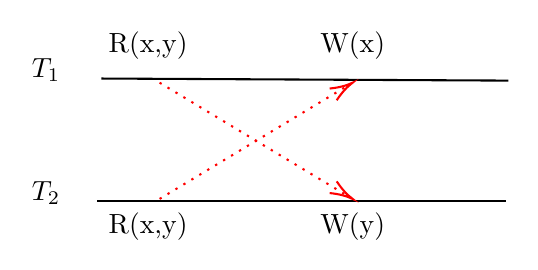
\begin{tikzpicture}[x=0.75pt,y=0.75pt,yscale=-1,xscale=1]
%uncomment if require: \path (0,300); %set diagram left start at 0, and has height of 300

%Straight Lines [id:da9500410641573396] 
\draw    (173.45,115) -- (369.56,116) ;
%Straight Lines [id:da7796185686481738] 
\draw    (171.56,174) -- (368.62,174) ;
%Straight Lines [id:da05192673528173475] 
\draw [color={rgb, 255:red, 255; green, 0; blue, 0 }  ,draw opacity=1 ] [dash pattern={on 0.84pt off 2.51pt}]  (201.56,173) -- (292.85,118.03) ;
\draw [shift={(294.56,117)}, rotate = 148.95] [color={rgb, 255:red, 255; green, 0; blue, 0 }  ,draw opacity=1 ][line width=0.75]    (10.93,-3.29) .. controls (6.95,-1.4) and (3.31,-0.3) .. (0,0) .. controls (3.31,0.3) and (6.95,1.4) .. (10.93,3.29)   ;
%Straight Lines [id:da10349511339666284] 
\draw [color={rgb, 255:red, 255; green, 0; blue, 0 }  ,draw opacity=1 ] [dash pattern={on 0.84pt off 2.51pt}]  (201.56,117) -- (292.85,171.97) ;
\draw [shift={(294.56,173)}, rotate = 211.05] [color={rgb, 255:red, 255; green, 0; blue, 0 }  ,draw opacity=1 ][line width=0.75]    (10.93,-3.29) .. controls (6.95,-1.4) and (3.31,-0.3) .. (0,0) .. controls (3.31,0.3) and (6.95,1.4) .. (10.93,3.29)   ;

% Text Node
\draw (138.5,104) node [anchor=north west][inner sep=0.75pt]   [align=left] {$T_1$};
% Text Node
\draw (138.5,163) node [anchor=north west][inner sep=0.75pt]   [align=left] {$T_2$};
% Text Node
\draw (277.56,178) node [anchor=north west][inner sep=0.75pt]   [align=left] {W(y)};
% Text Node
\draw (175.56,91) node [anchor=north west][inner sep=0.75pt]   [align=left] {R(x,y)};
% Text Node
\draw (175.56,178) node [anchor=north west][inner sep=0.75pt]   [align=left] {R(x,y)};
% Text Node
\draw (277.56,91) node [anchor=north west][inner sep=0.75pt]   [align=left] {W(x)};


\end{tikzpicture}


\caption{G2-item violation between $T_1$ and $T_2$, (rw, rw) resulting in an invalid state.}
\end{figure}

